\chapter{\selectlanguage{greek}Μεθοδολογία}
Στο κεφάλαιο αυτό περιγράφεται η προσέγγιση μας στην παραγωγή κώδικα χρησιμοποιώντας αναδραστικά νευρωνικά δίκτυα.
Εμπνεόμαστε από το \en{blog post} του \en{Andrej Karpathy}\footnote{\en{\url{http://karpathy.github.io/2015/05/21/rnn-effectiveness/}}}, στο οποίο χρησιμοποιείται μια σχετικά απλή δομή \en{RNN} με \en{LSTM} στοιχεία η οποία εκπαιδεύεται στα έργα του \en{Shakespeare}, κατά χαρακτήρα, και παράγει παρόμοιο κείμενο.
Χρησιμοποιούμε το ίδιο μοντέλο, εκπαιδευμένο σε κώδικα \en{JavaScript}.
Προτείνουμε μία επέκταση του προηγούμενου μοντέλου που χρησιμοποιεί \en{a priori} γνώση για τον κώδικα, με σκοπό να βελτιώσουμε τις επιδόσεις πρόβλεψης του μοντέλου και να εξετάσουμε τη διαίσθηση πως με περισσότερη χρήσιμη πληροφορία ο παραγόμενος κώδικας θα είναι ποιοτικότερος.
Εξετάζουμε τα μοντέλα σε 2 διαφορετικά σετ δεδομένων.
Παρακάτω ακολουθεί αναλυτική παρουσίαση της μεθόδου, την οποία χωρίζουμε σε 3 στάδια: 1) προ-επεξεργασία, 2) εκπαίδευση και 3) παραγωγή.

\section{Τα μοντέλα}

\subsection{Τα Αναδραστικά Νευρωνικά Δίκτυα ως Μοντέλα Παραγωγής}
Ο στόχος της μοντελοποίησης γλώσσας κατά χαρακτήρα (χωρίς να αναφερόμαστε απαραίτητα στην προγραμματιστική γλώσσα) είναι να προβλέψει τον επόμενο χαρακτήρα σε μία ακολουθία.
Δεδομένης μιας εκπαιδευτικής ακολουθίας $(x_1, x_2, ..., x_T)$, τα αναδραστικά νευρωνικά δίκτυα χρησιμοποιούν τις εξόδους τους $(ο_1, ο_2, ..., ο_T)$ για να πάρουν κατανομές προβλέψεων της μορφής $P(x_{t+1}|x_{\leq{t}}) = P(softmax(o_t))$, όπου η κατανομή <<\en{softmax}>> ορίζεται: $P(softmax(o_t) = j) = exp(o_t^{(j)}/\sum_k exp(o_t^{(k)})$.
Ο στόχος που χρησιμοποιείται για την μοντελοποίηση της γλώσσας είναι η μεγιστοποίηση της λογαριθμικής πιθανότητας της εκπαιδευτικής ακολουθίας $\sum_{t=0}^{T-1}logP(x_{t+1}|x_{\leq{t}})$.
Όπως και στην εργασία των \en{Graves et al.} \cite{Graves2013}, εισάγουμε στοχαστικότητα δειγματοληπτώντας από την έξοδο του νευρωνικού δικτύου και δίνοντας την τυχαία επιλογή μας ως είσοδο, την επόμενη χρονική στιγμή.

\subsection{Μοντέλο \en{char-rnn}}

Το πρώτο μοντέλο είναι ένα αναδραστικό νευρωνικό δίκτυο με 3 κρυμμένα επίπεδα στοιχείων \en{LSTM}.
Κάθε στιγμή το σύστημα δέχεται χαρακτήρες κώδικα σε μορφή διανυσμάτων  \en{\textit{one-hot}} (διανύσματα με όλα τα στοιχεία 0 εκτός από το στοιχείο εκείνο που αντιστοιχεί στον χαρακτήρα και παίρνει την τιμή 1).
Ενημερώνει την εσωτερική του κατάσταση και εξάγει μια πρόβλεψη για τον επόμενο χαρακτήρα.
Οι προβλέψεις του \en{char-rnn} είναι κατανομές του λεξιλογίου, που στην περίπτωση μας αποτελείται από χαρακτήρες.
Έστω ότι έχουμε το λεξιλόγιο \en{A, B, C, T}.
Αν θέλουμε να εκπαιδεύσουμε το σύστημα στην ακολουθία <<\en{BCAT}>>, δίνουμε ένα χαρακτήρα τη φορά και θέλουμε να μεγιστοποιηθούν οι υπογραμμισμένες πιθανότητες (Σχήμα \ref{fig:char-rnn}). Στη διαδικασία της παραγωγής (διακεκομμένες γραμμές) δειγματοληπτούμε από τις κατανομές εξόδου για να αποφασίσουμε τον επόμενο χαρακτήρα που δίνεται στο σύστημα. 


\begin{figure}[h]
	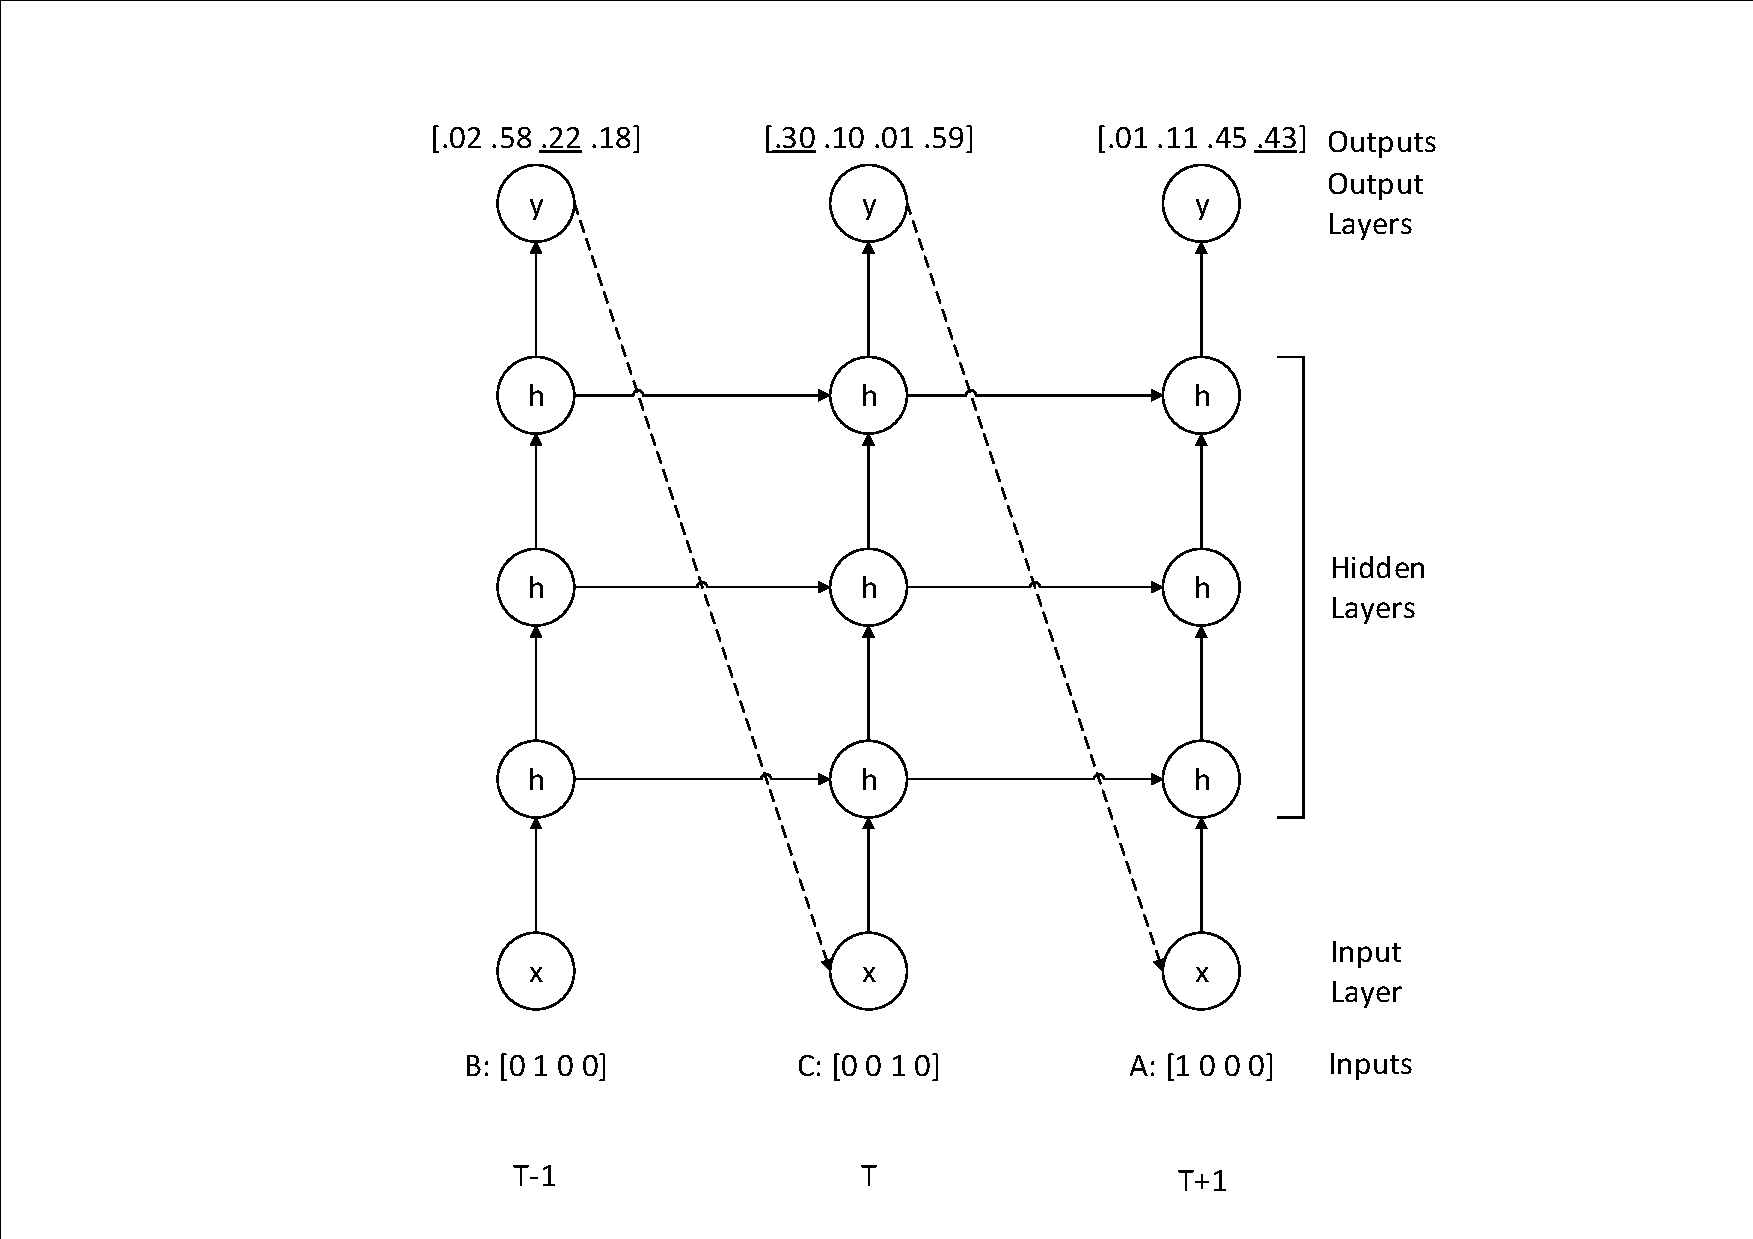
\includegraphics[width=\textwidth, trim = 4 4 4 4, clip, keepaspectratio]{images/char-rnn.pdf}
	\centering 
	\caption{Το μοντέλο \en{char-rnn} ανεπτυγμένο στο χρόνο.}
	\label{fig:char-rnn}
\end{figure}

\subsection{Μοντέλο \en{labeled-char-rnn}}

Το δεύτερο μοντέλο είναι επίσης ένα αναδραστικό νευρωνικό δίκτυο με 3 κρυμμένα επίπεδα στοιχείων \en{LSTM}. 
Εκτός από ακολουθίες χαρακτήρων, το μοντέλο αυτό δέχεται και πληροφορία για το είδος του χαρακτήρα. 
Αντίστοιχα οι έξοδοι του, εκτός από προβλέψεις για τον χαρακτήρα, περιέχουν και προβλέψεις για το είδος του χαρακτήρα. Με τον τρόπο αυτό θα εξετάσουμε κατά πόσο τα \en{RNNs} μπορούν να εκμεταλλευτούν \en{a priori} γνώσεις για τον κώδικα. Σημειώνεται πως η συνάρτηση επιδόσεων αυτού του μοντέλου είναι γραμμικός συνδυασμός των επιμέρους επιδόσεων πρόβλεψης χαρακτήρα και είδους χαρακτήρα.

Έστω το λεξιλόγιο \en{A, B, C, T}.
Έστω επίσης πως δίνουμε το είδος των χαρακτήρων αυτών στο σύστημα με βάση το αν είναι φωνήεντα ή σύμφωνα.
Για την εκπαιδευτική ακολουθία  <<\en{BCAT}>> δίνουμε την κατάλληλη είσοδο όπως στο σχήμα \ref{fig:l-char-rnn}.
Θέλουμε να μεγιστοποιηθούν και πάλι οι υπογραμμισμένες πιθανότητες. Για την παραγωγή του επόμενου χαρακτήρα και του είδους του, δειγματοληπτούμε από κάθε κατανομή εξόδου ξεχωριστά.

\begin{figure}[h]
	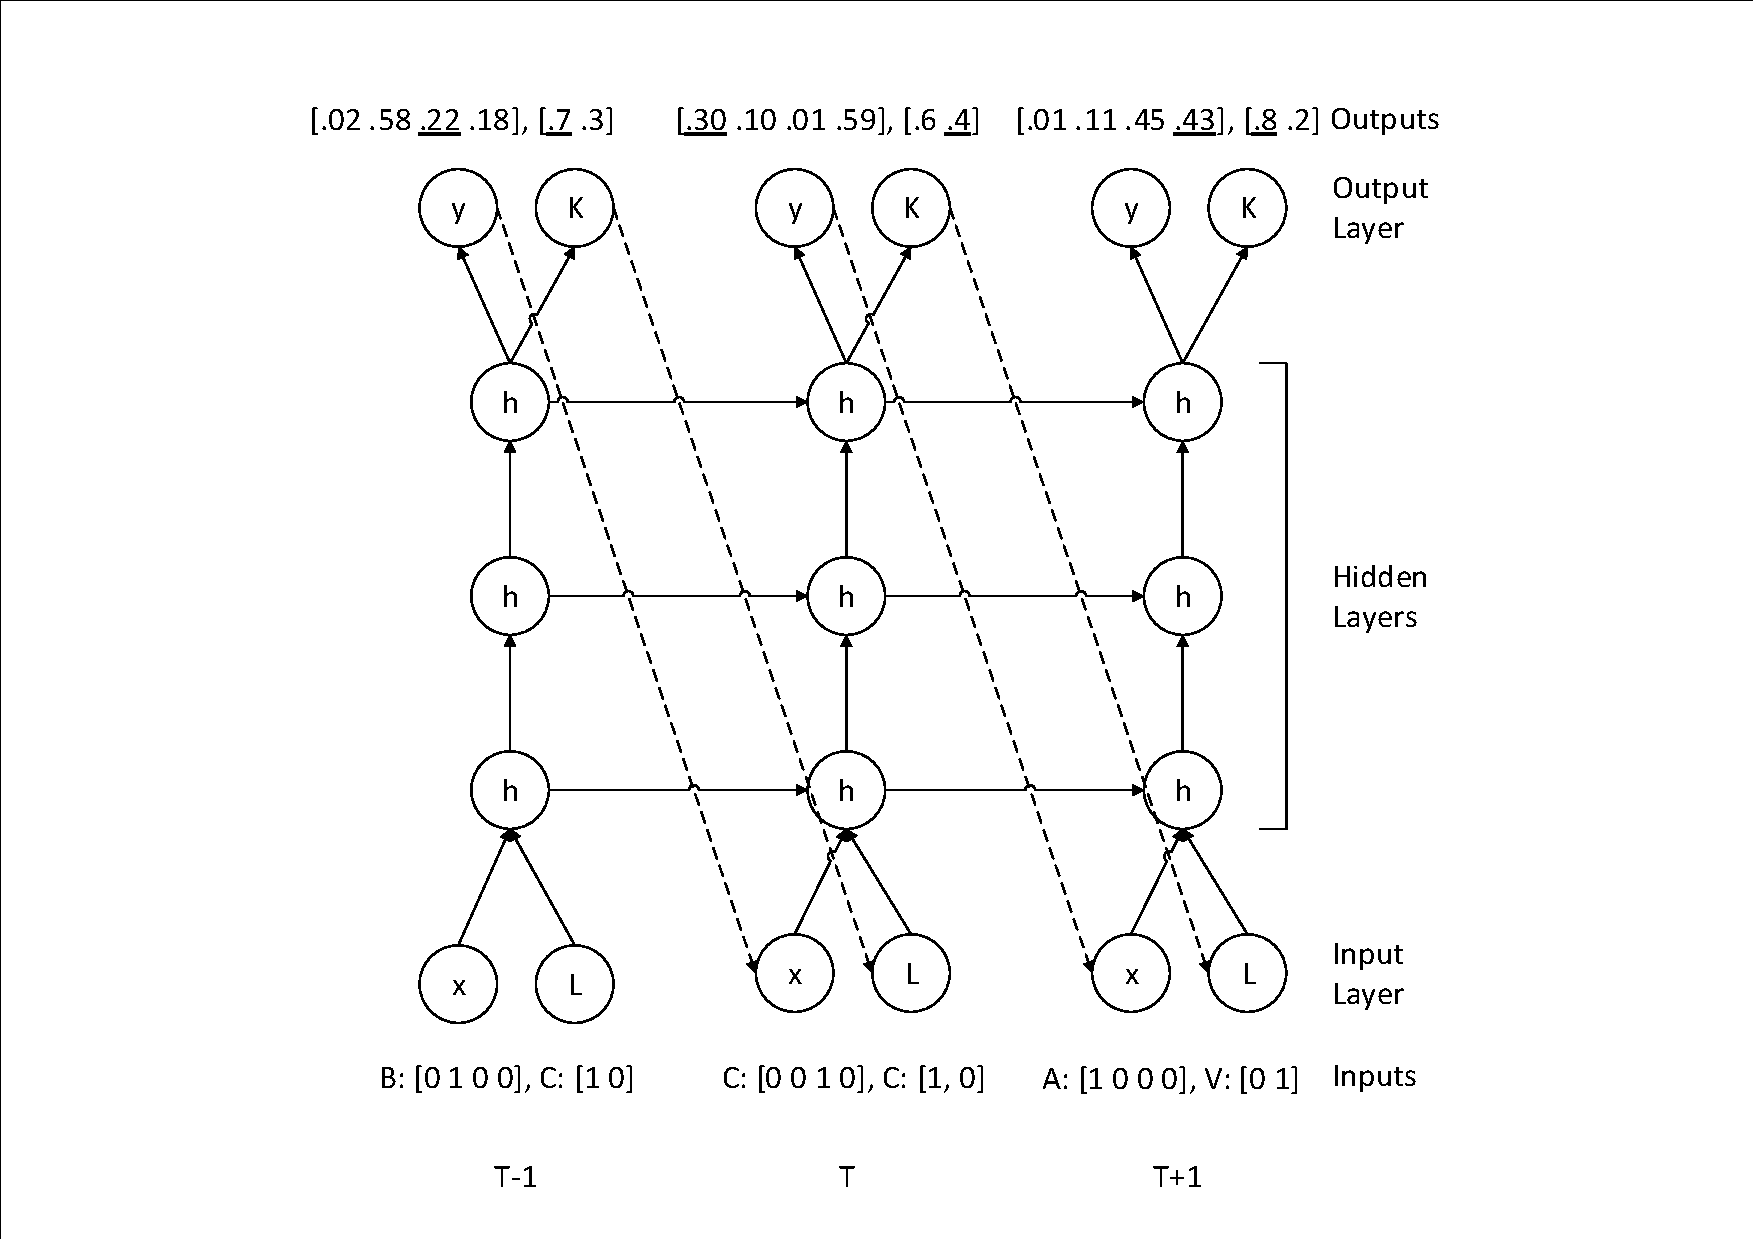
\includegraphics[width=\textwidth, trim = 4 4 4 4, clip, keepaspectratio]{images/l-char-rnn.pdf}
	\centering 
	\caption{Το μοντέλο \en{labeled-char-rnn} ανεπτυγμένο στο χρόνο.}
	\label{fig:l-char-rnn}
\end{figure}

\section{Προ-επεξεργασία}

Ο κορμός της διαδικασίας της προ-επεξεργασίας είναι ίδιος και για τα δύο σετ δεδομένων. 
Αρχικά αναζητούμε τα αρχεία με κατάληξη <<\en{.js}>> διασχίζοντας σειριακά όλους τους φακέλους των \en{projects}, εκτός από αυτούς που αφορούν \en{testing} και \en{localization}.
Ο έλεγχος για το τελευταίο γίνεται απλοϊκά, ελέγχουμε δηλαδή αν οι φάκελοι φέρουν τα συνήθη ονόματα που χρησιμοποιούνται για τέτοιου είδους φακέλους.
Ο μη ενδελεχής έλεγχος καταφέρνει να αφαιρέσει την πλειοψηφία των επαναλαμβανόμενων αρχείων αφήνοντας ένα μικρό ποσοστό να περάσει.
Αυτό έχει ως αποτέλεσμα να εμπλουτιστεί η εκπαίδευση του νευρωνικού, χωρίς όμως να μονοπωλείται το ενδιαφέρον από αρχεία που περιέχουν τετριμμένο κώδικα.
Στη συνέχεια, με τη βοήθεια ενός εργαλείου ανάλυσης της σύνταξης και γραμματικής προγραμματιστικών γλωσσών (ονόματι \en{\textit{linguist}}\footnote{\en{\url{https://github.com/github/linguist/}}}) προχωράμε στο περαιτέρω φιλτράρισμα αρχείων.
Συγκεκριμένα, εξαιρούμε αρχεία που έχουν την κατάληξη <<\en{.js}>> αλλά δεν είναι αρχεία κειμένου και αρχεία που είναι αυτόματα παραγόμενα και αποτελούν παραπροϊόν της διαδικασίας ανάπτυξης λογισμικού σε \en{JavaScript}.

\selectlanguage{english}
\lstinputlisting[language=JavaScript, caption={\tg{Αρχείο κώδικα πριν το }\en{minification}}]{code/beforemin.js}
\selectlanguage{greek}

\selectlanguage{english}
\lstinputlisting[language=JavaScript, caption={\tg{Αρχείο κώδικα μετά το }\en{minification}}]{code/aftermin.js}
\selectlanguage{greek}

Αφού επιλέξουμε τα αρχεία τα οποία θα αποτελούν το σετ δεδομένων μας προχωράμε στη διαδικασία της ελαχιστοποίησης του κώδικα (\en{minification, minimisation}).
Η ελαχιστοποίηση κώδικα, είναι η διαδικασία αφαίρεσης περιττών χαρακτήρων από των πηγαίο κώδικα, χωρίς να αλλάζει η λειτουργικότητά του. Τέτοιοι χαρακτήρες είναι τα κενά, τα σύμβολα αλλαγής παραγράφου, τα σχόλια και άλλα. Εδώ χρησιμοποιήθηκε το εργαλείο \en{\textit{jsmin}}\footnote{\en{\url{http://www.crockford.com/javascript/jsmin.html}}}. Οι κώδικες 4.1, 4.2 δείχνουν ένα αρχείο κώδικα πριν και μετά το \en{minification}.

Με την επιλογή αυτή προσπαθούμε να αφαιρέσουμε την περιττή πληροφορία απο τα δεδομένα μας, ώστε να είναι πιο εύκολο για το μοντέλο να αποτυπώσει τις σημαντικές σχέσεις ανάμεσα στους διάφορους χαρακτήρες.
Μετά το \en{minification} προσθέτουμε 2 ειδικούς χαρακτήρες για την αρχή και το τέλος κάθε αρχείου. Σημειώνεται πως θεωρούμε πως τα αρχεία ειναι \en{extended ASCII} κωδικοποιημένα και στην ουσία διαβάζουμε \en{bytes}.

Για την εκπαίδευση του μοντέλου \en{labeled-char-rnn} χρειάζεται να προετοιμάσουμε με ανάλογο τρόπο την πληροφορία για το είδος των χαρακτήρων. Για το σκοπό αυτό, χρησιμοποιούμε ένα άλλο εργαλείο ανάλυσης σύνταξης και γραμματικής προγραμματιστικών γλωσσών που φέρει το όνομα \en{\textit{pygments}}\footnote{\en{\url{http://pygments.org}}}.
Η επιλογή για τον διαχωρισμό των ειδών βασίζεται στα αυθαίρετα συντακτικά δέντρα (\en{abstract syntax trees}) της \en{JavaScript}, είναι όμως απλουστευμένη και δε χρησιμοποιεί δομές δέντρων, αλλά απλών διανυσμάτων.
Ο διαχωρισμός των χαρακτήρων γίνεται ανάμεσα στις ακόλουθες κλάσεις: \en{(\textbf{K}eyword, \textbf{N}umber, \textbf{R}egex, \textbf{S}tring, \textbf{O}perator, \textbf{P}unctuator, \textbf{I}dentifier).}

Οι χαρακτήρες και τα είδη τους αποθηκεύονται ως λίστες από αλφαριθμητικά στοιχεία ώστε να είναι διαθέσιμα ανά πάσα στιγμή στην εκπαιδευτική διαδικασία.
Προφανώς υπάρχει χρονική αντιστοιχία μεταξύ των αρχείων που περιέχουν της ακολουθίες χαρακτήρων με τα αρχεία που περιέχουν το είδος κάθε χαρακτήρα, όπως στα παραδείγματα του πίνακα \ref{label-example}.
Συνηθίζεται σε τέτοιου είδους προβλήματα να <<\tg{ανακατεύονται}>> οι ακολουθίες αλφαριθμητικών χαρακτήρων με σκοπό την .
Στα προβλήματα μάθησης έχουμε τη δυνατότητα να <<\tg{ανακατεύουμε}>> το σετ δεδομένων με σκοπό την γρηγορότερη/καλύτερη εκπαίδευση των μοντέλων.
Επειδή το ζητούμενο μας στη διπλωματική αυτή είναι η παραγωγή κώδικα, και η σειρά των ακολουθιών είναι άρρηκτα συνδεδεμένη με τη λειτουργικότητα και την ουσία των προγραμμάτων, δεν προχωράμε σε αυτή την επιλογή.  

\begin{table}[]
\centering
\caption{Παράδειγμα αντιστοιχίας χαρακτήρων με το είδος τους σε μια ακολουθία}
\label{label-example}
\begin{tabularx}{\textwidth}{|l|XXXXXXXXXXXXXXXXXXXXX|}
\hline
\en{String 1} & \en{v} & \en{a} & \en{r} &   & \en{a} & = & 1 & \en{;} & \en{f} & \en{u} & \en{n} & \en{c} & \en{t} & \en{i} & \en{o} & \en{n} &   & \en{f} & \en{(} & \en{A} & \en{)} \\ \hline
\en{Label 1}  & \en{K} & \en{K} & \en{K} & \en{P} & \en{I} & \en{O} & \en{N} & \en{P} & \en{K} & \en{K} & \en{K} & \en{K} & \en{K} & \en{K} & \en{K} & \en{K} & \en{P} & \en{I} & \en{P} & \en{I} & \en{P} \\ \hline
\hline
\en{String 2} & \{ & \en{r} & \en{e} & \en{t}  & \en{u} & \en{r} & \en{n} &  & < & \en{o} & \en{k} &  > & \en{;} & \} & \en{c} & = & \en{f} & \en{(} & \en{1} &\en{0} & \en{)} \\ \hline
\en{Label 2}  & \en{P} & \en{K} & \en{K} & \en{K} & \en{K} & \en{K} & \en{K} & \en{P} & \en{S} & \en{S} & \en{S} & \en{S} & \en{P} & \en{P} & \en{I} & \en{O} & \en{I} & \en{P} & \en{N} & \en{N} & \en{P} \\ \hline
\end{tabularx}
\end{table}

\section{Εκπαίδευση}


Η εκπαίδευση γίνεται στο \en{training set} του καθενός από τα δύο σετ δεδομένων. 
Οι χαρακτήρες δίνονται ως \en{\textit{one-hot}} διανύσματα, με μήκος όσο και οι διαφορετικοί χαρακτήρες του σετ δεδομένων.
Χρησιμοποιείται η τεχνική του \en{dropout}, ενώ ο αλγόριθμος που χρησιμοποιείται για την ελαχιστοποίηση του λάθους είναι ο \en{TBPTT}.
Η συνάρτηση λάθους είναι η \en{cross-entropy loss function}: $\sum_x p(x) \log{q(x)}$, όπου $p(x)$ είναι η πραγματική κατανομή των χαρακτήρων και $q(x)$ η προβλεπόμενη κατανομή χαρακτήρων του μοντέλου.
Η συνάρτηση αυτή χρησιμοποιείται στην πλειοψηφία της σύγχρονης βιβλιογραφίας και εμπειρικά έχει καλά αποτελέσματα στην εκπαίδευση των αναδραστικών νευρωνικών δικτύων.
Εξίσου ευρεία χρήση συναντά και η συνάρτηση \en{\textit{rmsprop}} που χρησιμοποιούμε για τη βελτιστοποίηση του \en{gradient descent}.

Η εκπαίδευση του αναδραστικού νευρωνικού δικτύου γίνεται, πιο περιγραφικά ως εξής: δείχνουμε στο νευρωνικό δίκτυο ακολουθίες σταθερού μήκους, το οποίο προαποφασίζεται της εκπαίδευσης.
Ως αληθείς απαντήσεις δίνουμε ένα διάνυσμα ίσου μήκους με το προηγούμενο που περιέχει τους χαρακτήρες της επόμενης χρονικής στιγμής (κύλιση του διανύσματος κατά μία θέση).
Στην περίπτωση του μοντέλου  \en{labeled-char-rnn} με όμοιο τρόπο δίνονται και οι πληροφορίες σχετικά με το είδος των χαρακτήρων, μαζί με τους αντίστοιχους χαρακτήρες.
Με σκοπό την παραλληλοποίηση του προγράμματος, δίνουμε πολλά τέτοια παραδείγματα ταυτόχρονα.

Συνολικά εκπαιδεύουμε 4 διαφορετικά μοντέλα. Για κάθε \en{dataset} το αντίστοιχο \en{char-rnn} και \en{labeled-char-rnn} μοντέλο.
Για την εκπαίδευση των μοντέλων, πρέπει να αποφασιστεί ένα σύνολο παραμέτρων, που φέρουν σημαντική αξία για τις τελικές επιδόσεις του μοντέλου και την διάρκεια της εκπαίδευσης. Αυτές είναι:

\begin{itemize} 
\item Μήκος ακολουθίας \en{(Sequence length)}: Ο αριθμός χαρακτήρων που περιέχει μία ακολουθία.
\item Μέγεθος παρτίδας \en{(Batch size)}: Ο αριθμός των εκπαιδευτικών ακολουθιών που δίνονται παράλληλα στο μοντέλο.
\item Μέγεθους κρυμμένων επιπέδων \en{(Hidden state size)}: Ο αριθμός των στοιχείων \en{LSTM} που απαρτίζουν κάθε κρυφό επίπεδο.
\item Πιθανότητα \en{dropout}: Η πιθανότητα να κρατηθεί ένα στοιχείο στη διάρκεια τη εκπαίδευσης.
\item Αριθμός εποχών \en{(Epoch number)}: Ο αριθμός <<περασμάτων>> του τεστ δεδομένων.
\item Ρυθμός εκμάθησης \en{(Learning rate)}: Πόσο γρήγορα μαθαίνει το σύστημα από τα λάθη του.

\end{itemize}

Για την στρατηγική επιλογής και την ακριβή τιμή των υπερ-παραμέτρων θα μιλήσουμε στο Κεφάλαιο 5.

\section{Παραγωγή}

Το μοντέλο που επιλέγουμε για καθένα από τα πειράματα αποφασίζεται σύμφωνα με τις επιδόσεις του στην μετρική λάθους της εκπαίδευσης.
Για να είναι ευκολότερα ερμηνεύσιμα τα αποτελέσματα της εκπαίδευσης, θα χρησιμοποιούμε και την μετρική της <<\tg{ευστοχίας}>>.
Η ευστοχία είναι το ποσοστό επιτυχημένων προβλέψεων επόμενου χαρακτήρα σε μία παρτίδα.

Η διαδικασία παραγωγής κώδικα που περιγράψαμε γενικεύεται και για τα μοντέλα που περιέχουν πληροφορία για το είδος των χαρακτήρων.
Μπορούμε δηλαδή να δειγματοληπτούμε από την προβλεπόμενη κατανομή για τα είδη των χαρακτήρων και να χρησιμοποιούμε το αποτέλεσμα ως επόμενη είσοδο.
Μπορούμε επίσης να οδηγήσουμε έμμεσα το σύστημα, αρχικοποιώντας το με κώδικα της επιλογής μας. Αυτό αλλάζει την εσωτερική κατάσταση του μοντέλου και το <<προϊδεάζει>> για το τι κώδικας μπορεί να ακολουθεί. 
Επιπρόσθετα, κατά τη διάρκεια της δειγματοληψίας έχουμε τη δυνατότητα να επηρεάσουμε την κατανομή που προτείνει το μοντέλο.
Αυτό ελέγχει το μοντέλο ως προς τη <<σιγουριά>> του για τις προβλέψεις του και έχει τη δυνατότητα να κάνει τον παραγόμενο κώδικα, είτε πιο ντετερμινιστικό, είτε πιο ποικίλο.
Σημαντική ιδιότητα αυτής της προσθήκης είναι πως δίνει στο μοντέλο τη δυνατότητα να ξεφύγει από φαύλους κύκλους ντετερμινιστικών λαθών χάρη στην επιπλέον τυχαιότητα που εισάγεται.
Η συνάρτηση ονομάζεται \en{\textit{Softmax Temperature}} και είναι: 

\begin{ceqn}
\begin{align}
P = \frac{e^{y/T}}{\sum_{k = 1}^{n} e^{y_k/T}}
\end{align}
\end{ceqn}

Όπου $P$ είναι η νέα κατανομή, $y$ είναι η εξαγόμενη του νευρωνικού δικτύου πιθανοτική κατανομή και $n$ ο αριθμός των διαφορετικών στοιχείων προς πρόβλεψη. $T$ είναι η τιμή της θερμοκρασίας που επηρεάζει την  κατανομή.
Για τιμές μεγαλύτερες του 1, ο κώδικας γίνεται πιο ποικίλος, αλλά με περισσότερα λάθη.
Τιμές μικρότερες του 1 έχουν ως αποτέλεσμα το σύστημα να είναι πιο σίγουρο για τις προβλέψεις του.



